\documentclass{article}

\usepackage[colorlinks=true, urlcolor=blue]{hyperref}
\usepackage{minted}
\usepackage{graphicx}

\title{Basile Relatório Max-Heapfy}
\author{Mateus Felipe da Silveira Vieira}

\begin{document}
    \maketitle

    \centerline{Repositório Git: \url{https://github.com/habdig7oficial/max_heapfy.git}}

    \vspace{0.9cm}

    \centerline{\huge Código Heapsort Completo}

    \vspace{0.5cm}

    \begin{minted}{C}
#include "stdio.h"
#include "math.h"
#include "stdbool.h"

void print_vec(int *vec, int len){
    printf("[");
    for (int i = 0; i < len; i++){
        printf("%d, ", vec[i]);
    }
    printf("]\n"); 
}

void swap(int *a, int *b){
    int aux = *a;
    *a = *b;
    *b = aux;
}

bool max_heapfy(int *vec, int i, int len){
    bool parity = (i % 2) == 0;
    int index_father = (int)i / 2 + (parity? -1 : 0);
    int index_brother = i + (parity ? -1 : 1);
    printf("Root: vec[%d] = %d\n", index_father, vec[index_father]);
    printf("Leaf: vec[%d] = %d\n", i, vec[i]);
    printf("Brother: vec[%d] = %d\n", index_brother, vec[index_brother]);
    printf("\n");

    if(index_brother >= len){
        return false;
    }
    int max_child = (vec[i] >= vec[index_brother])? i : index_brother;
    if(vec[max_child] > vec[index_father]){
        swap(&vec[index_father], &vec[max_child]);

        printf("Troca: %d %d\n", vec[max_child], vec[index_father]);
        return true;
    }

    print_vec(vec, len);
    return false;
}

int main(){
    int vec[] = {2, 14, 6, 8, 5, 4, 3, 1, 7, 9, 6, 10, 17, 20, 12, 19};
    int len = sizeof(vec) / sizeof(int);
    print_vec(vec, len);

    for(int i = len - 1; i > 0; i -= 2){
        max_heapfy(vec, i, len);
    }

    printf("\n----------End max Heapfy----------\n");

    print_vec(vec, len);

    for(int i = len - 1; i > 0; i--){
        swap(&vec[0], &vec[i]);
        for(int j = 1; max_heapfy(vec, j, i); j += 2){
            print_vec(vec, len);
        }
    }


    print_vec(vec, len);
}
    \end{minted}



    \vspace{0.9cm}

    \centerline{\Large Print de Execução}

    \vspace{0.5cm}

    \centerline{\Huge Max-Heapfy}

    \begin{figure}
        \centering
        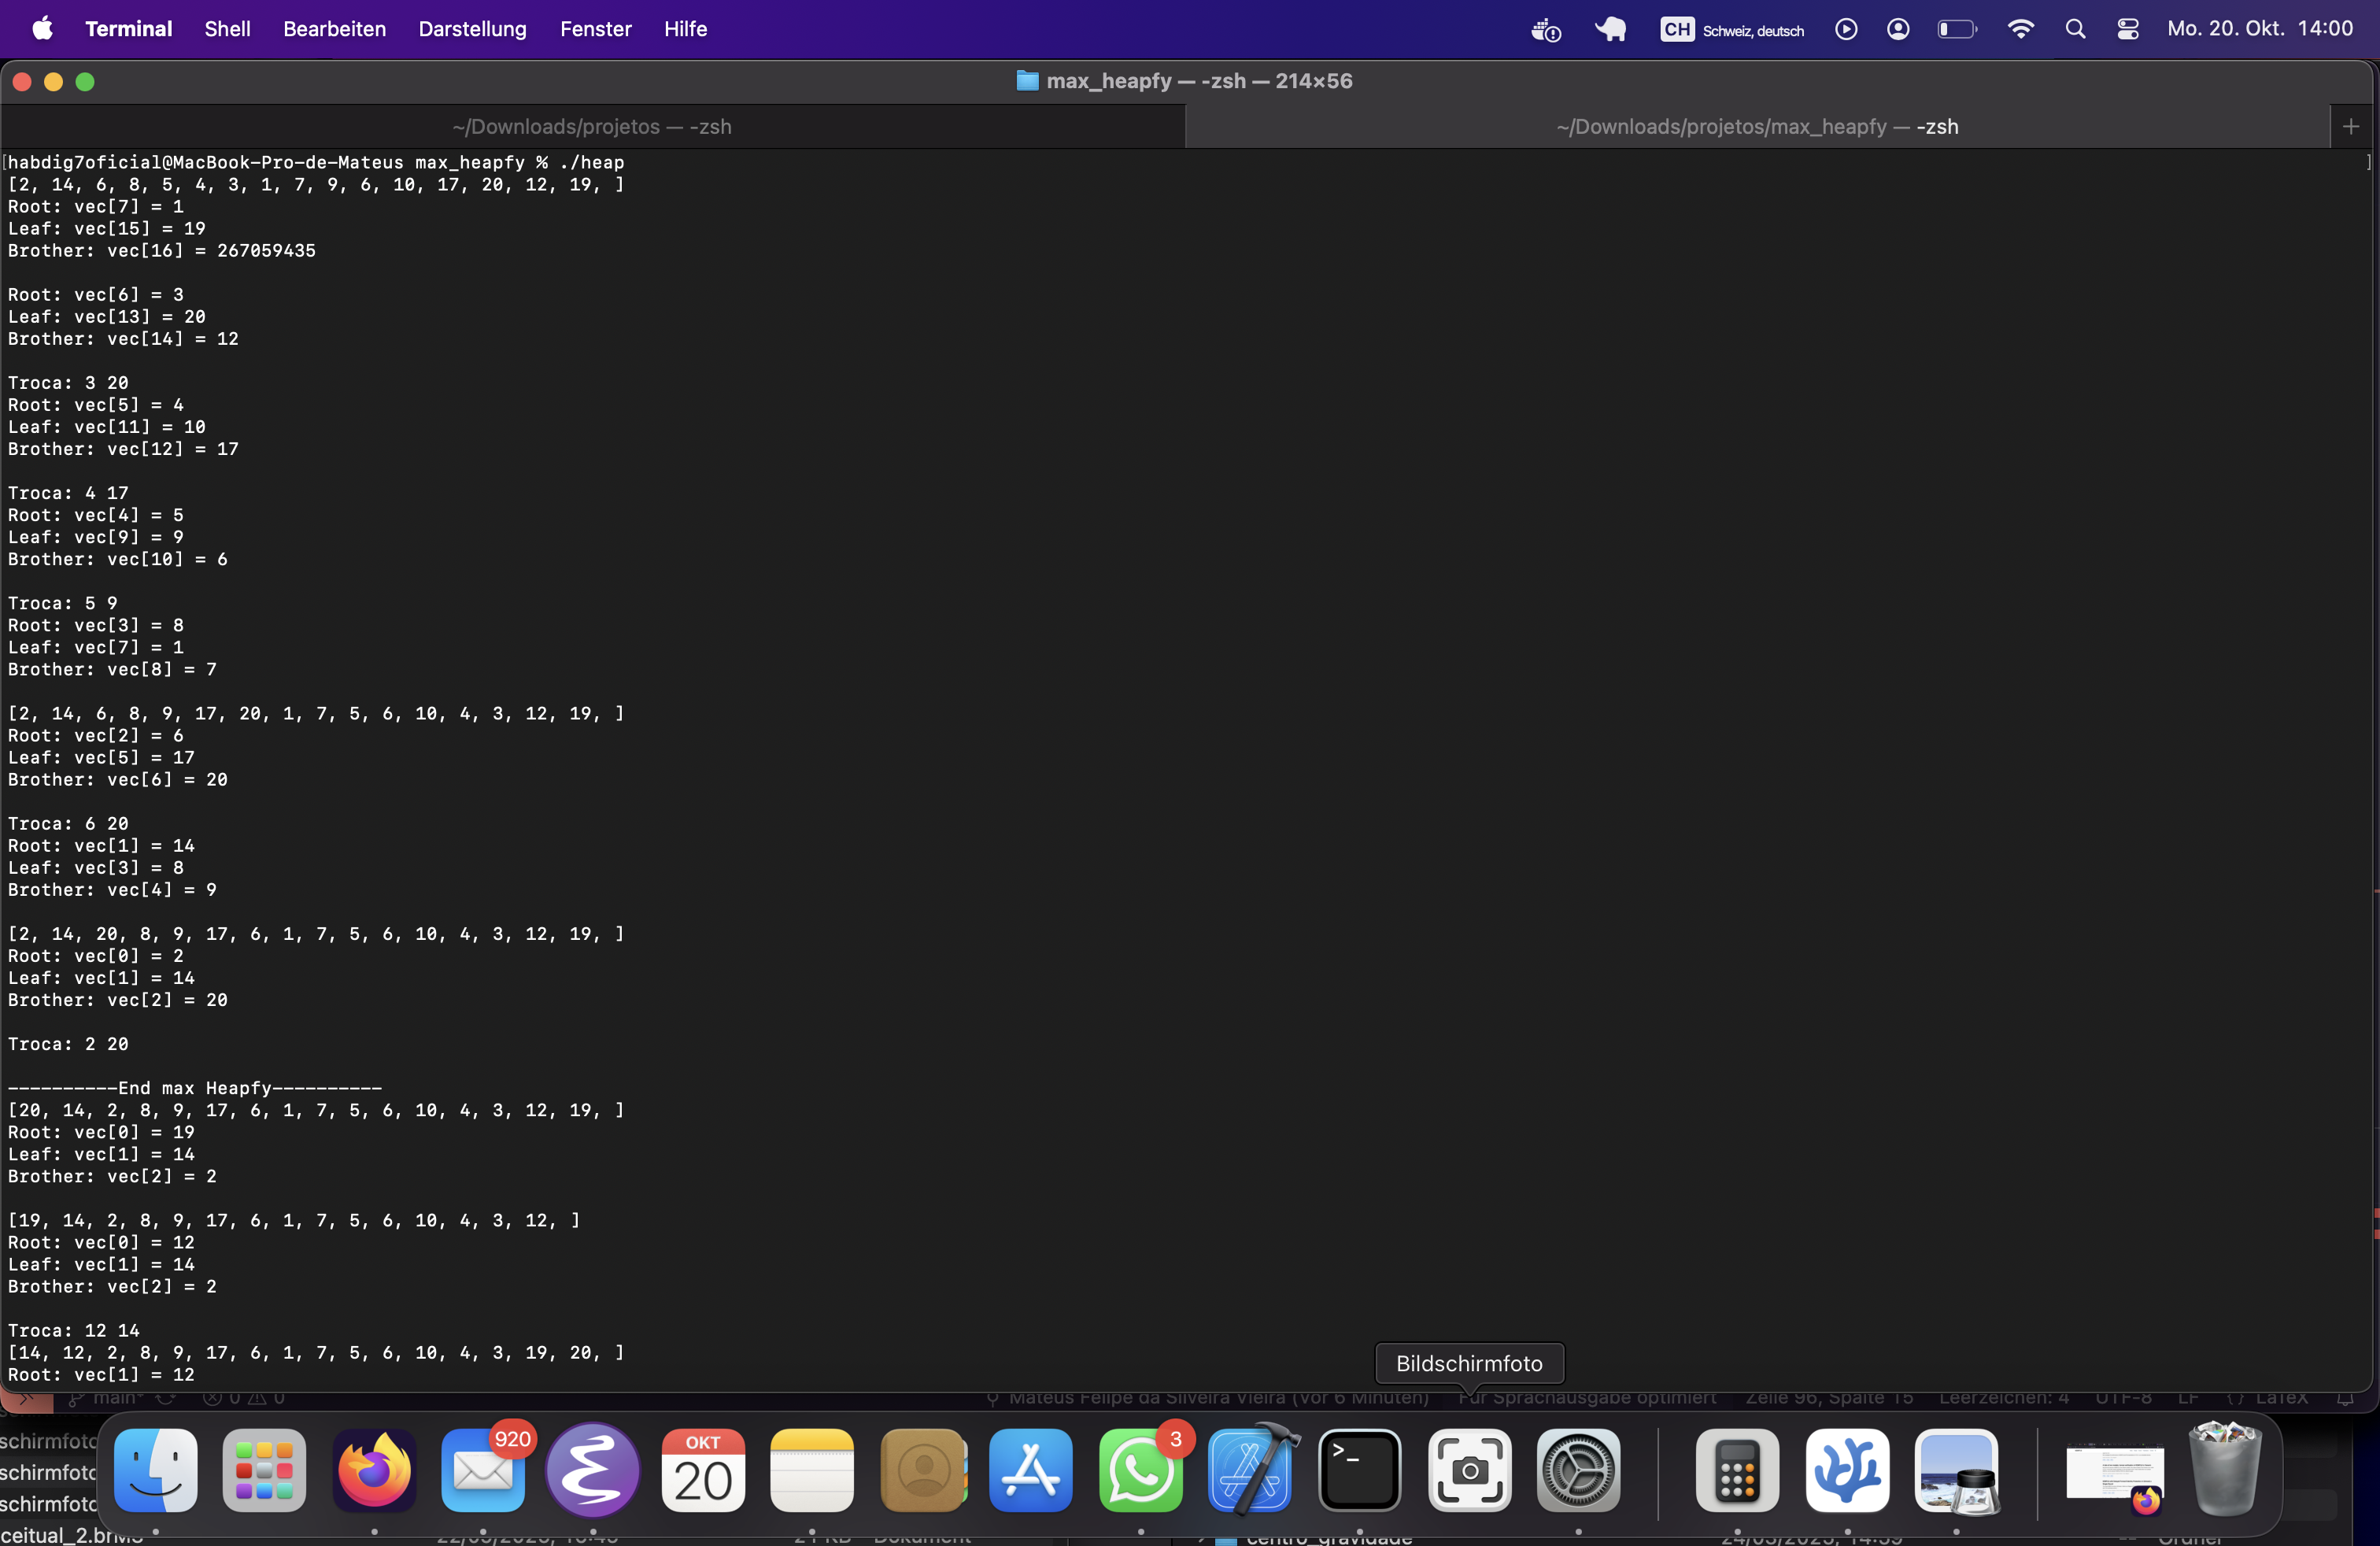
\includegraphics[width=1.3\linewidth]{max_heapfy.png}
        \caption{Max-Heapfy}
        \label{fig:fig1}
    \end{figure}

    \clearpage

    \centerline{\Huge Heap Sort}
    \clearpage

    \begin{figure}
        \centering
        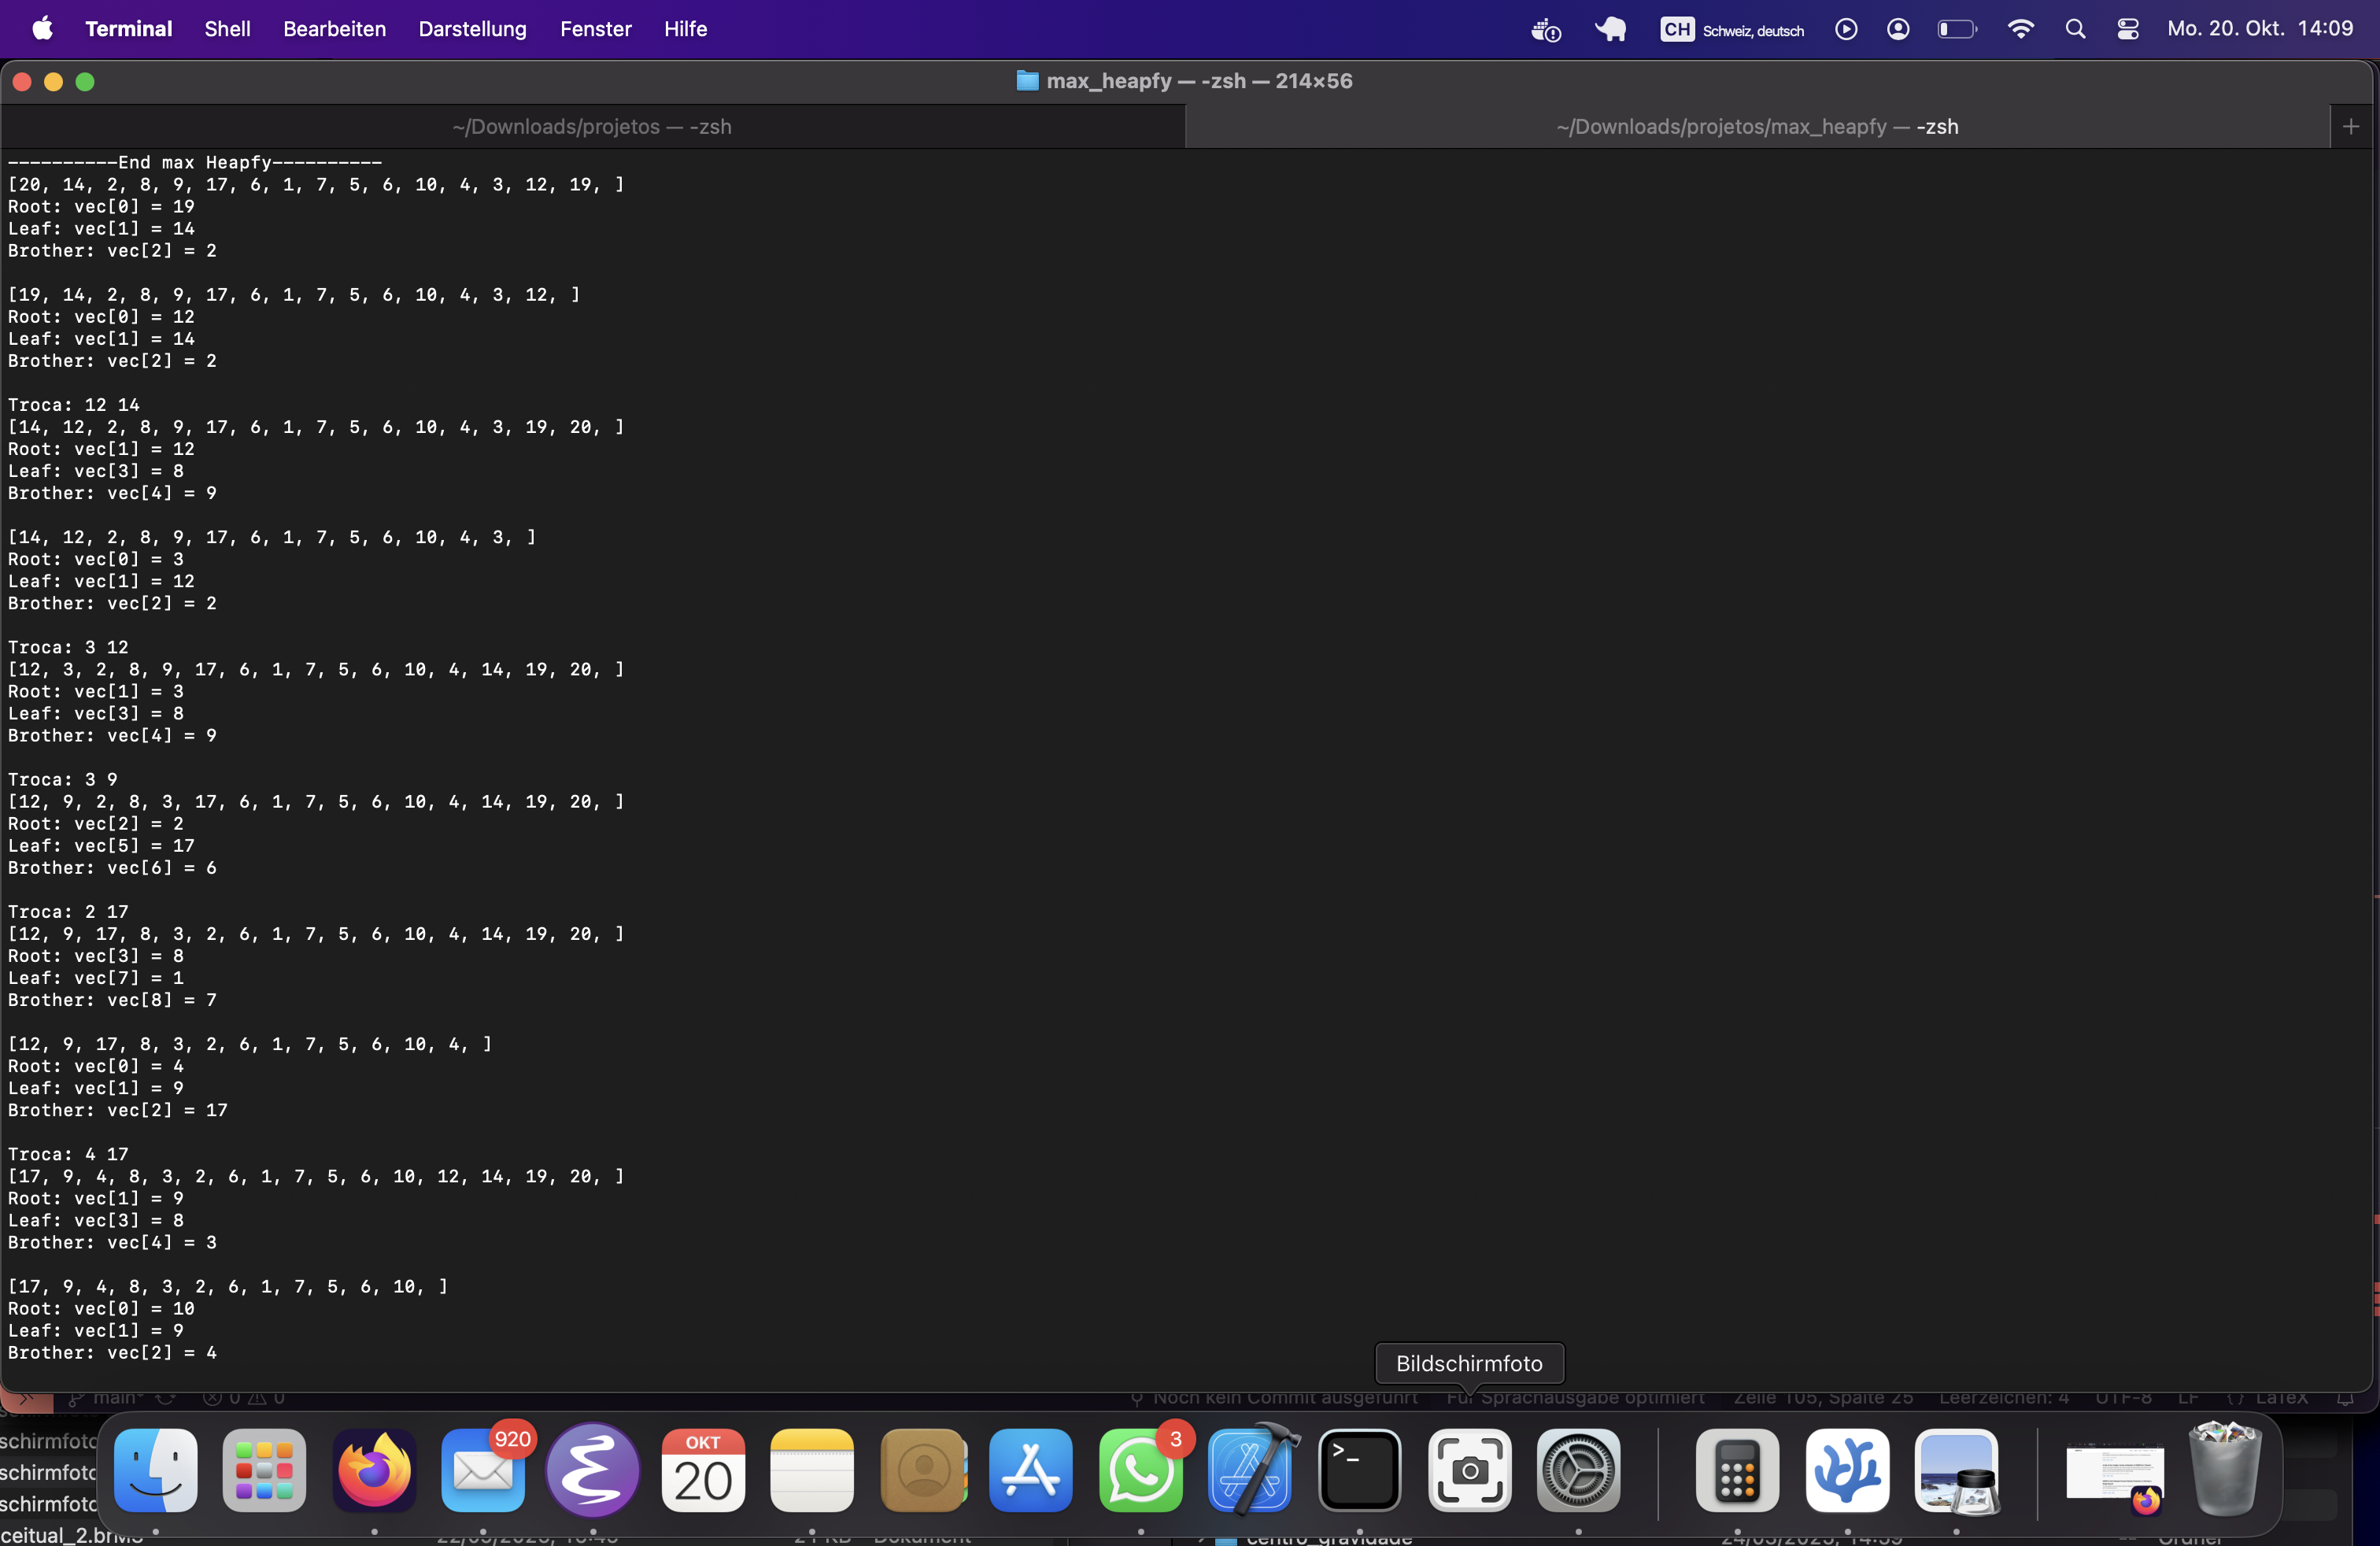
\includegraphics[width=1.3\linewidth]{heapsort1.png}
        \caption{Heap Sort, 1ª Página}
        \label{fig:myfig2}
    \end{figure}

    \begin{figure}
        \centering
        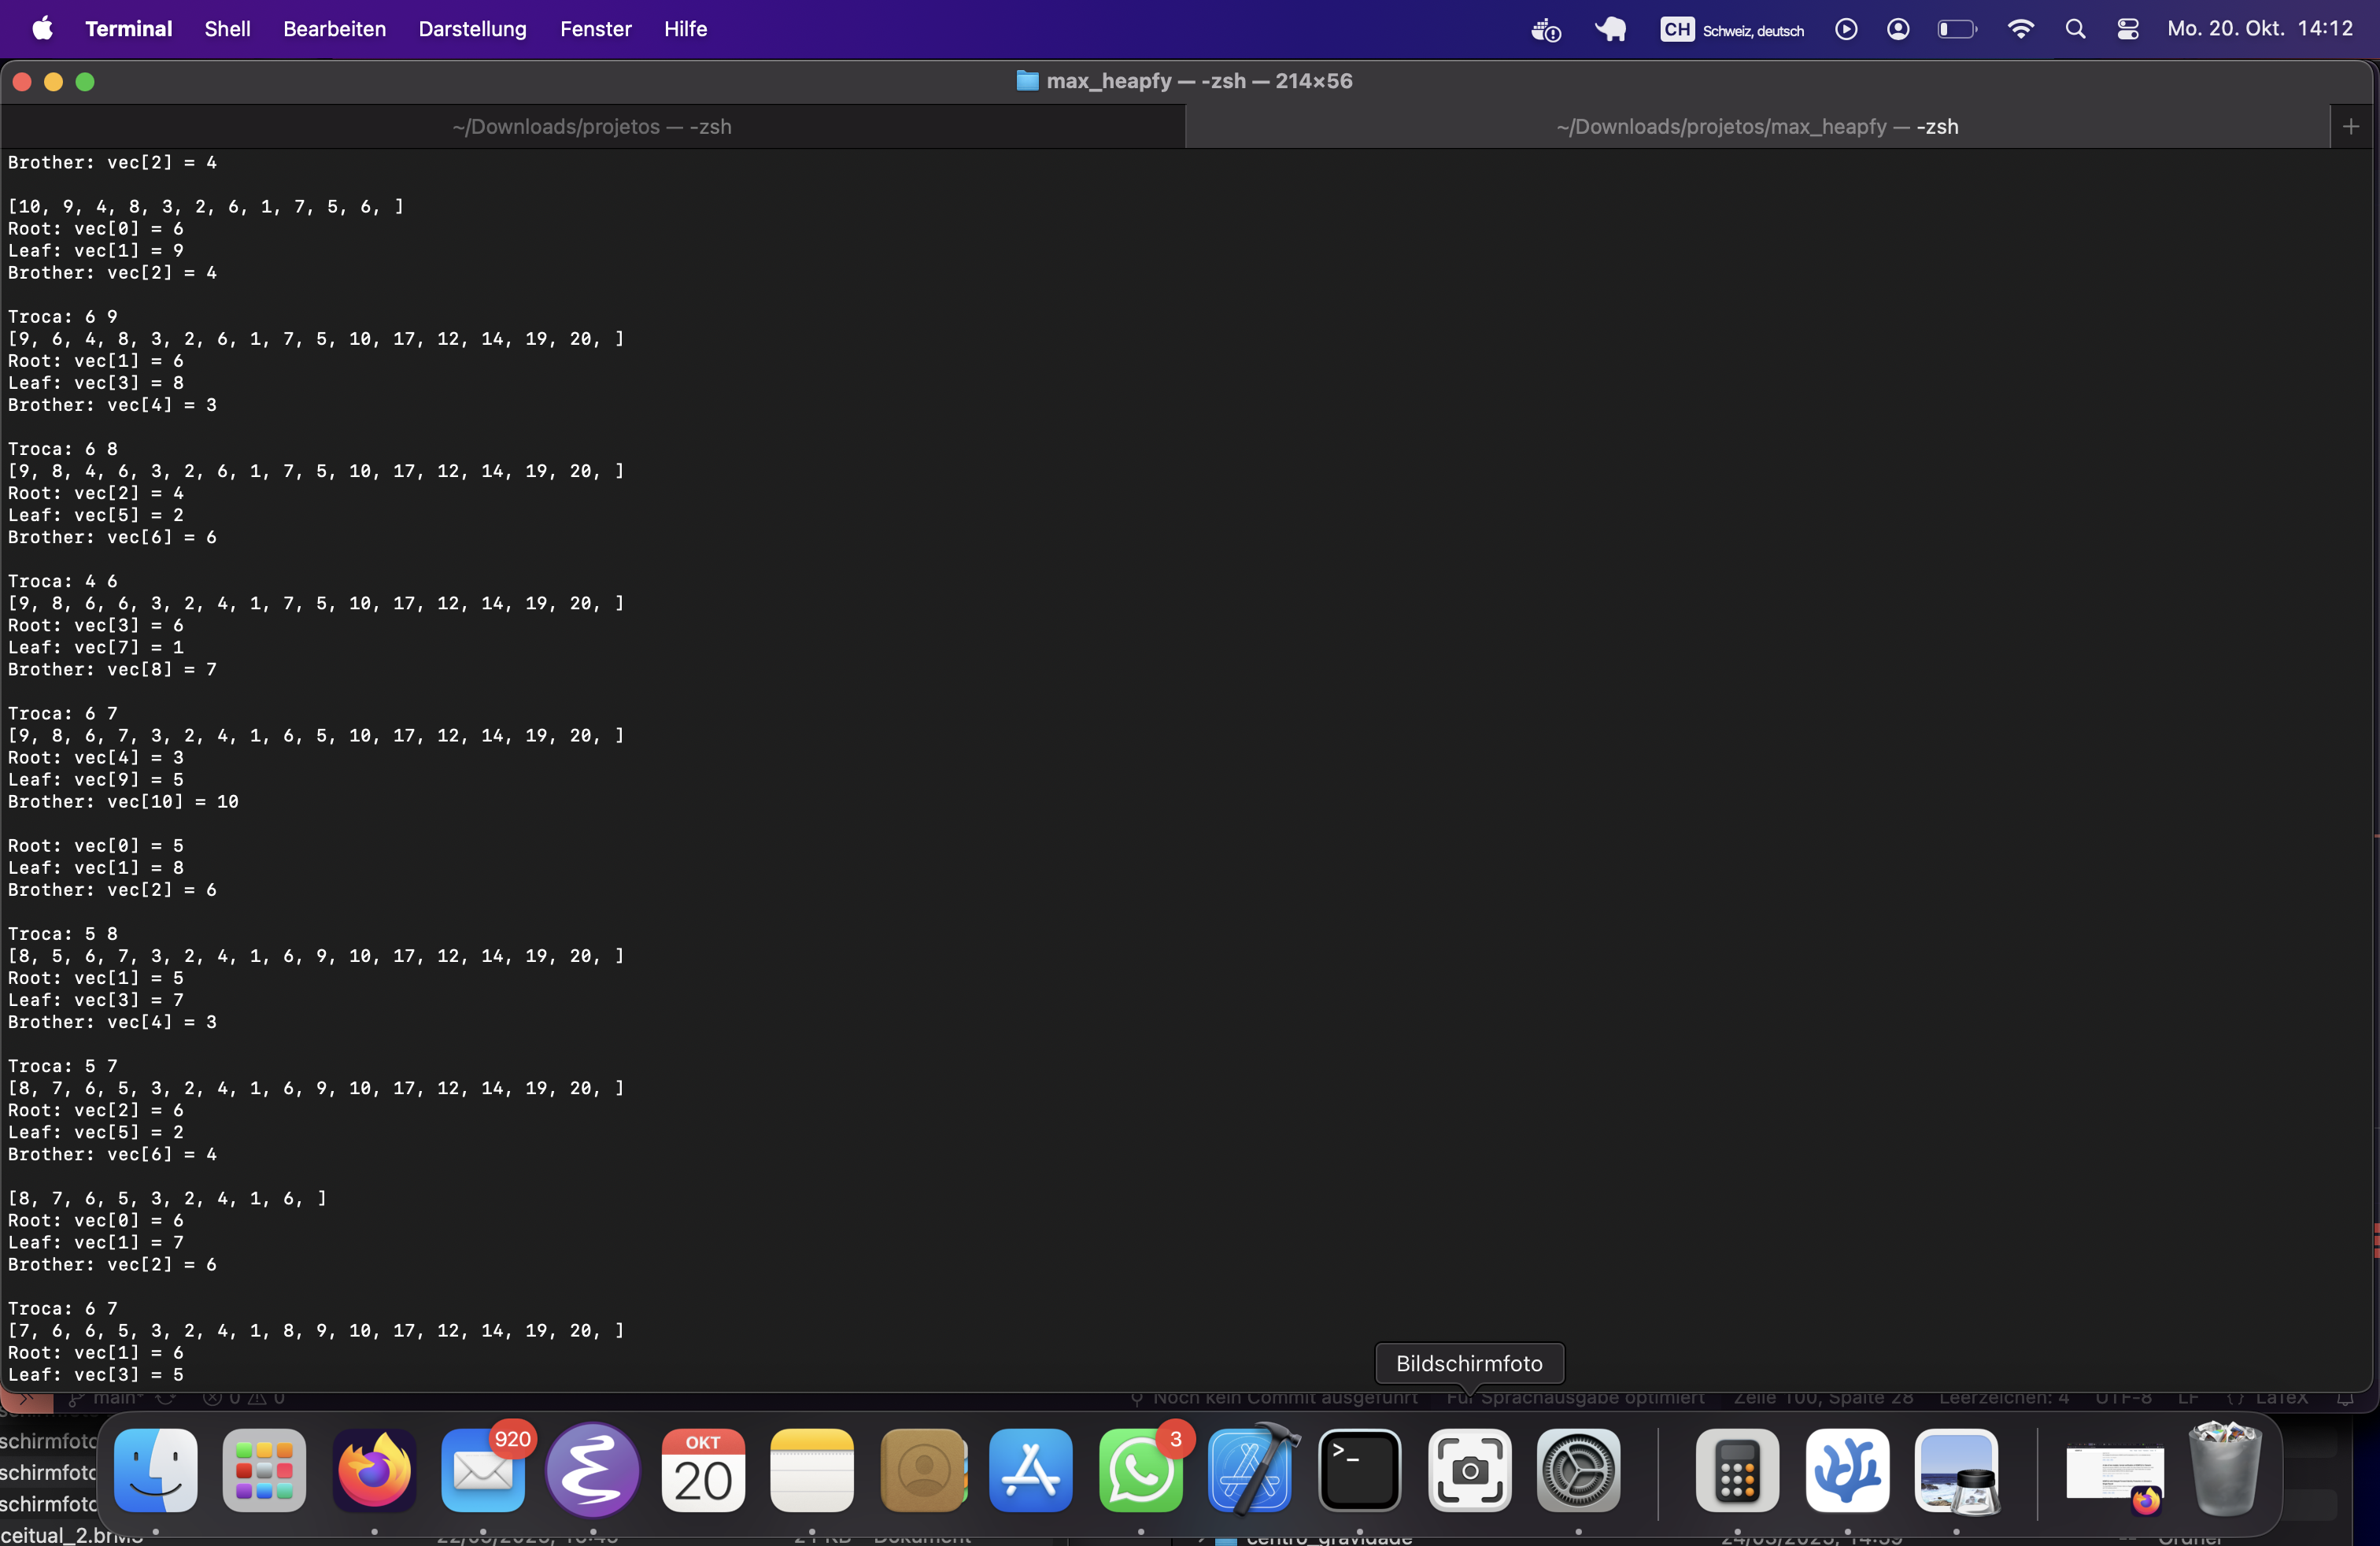
\includegraphics[width=1.3\linewidth]{heapsort2.png}
        \caption{Heap Sort, 2ª Página}
        \label{fig:myfig3}
    \end{figure}

    \begin{figure}
        \centering
        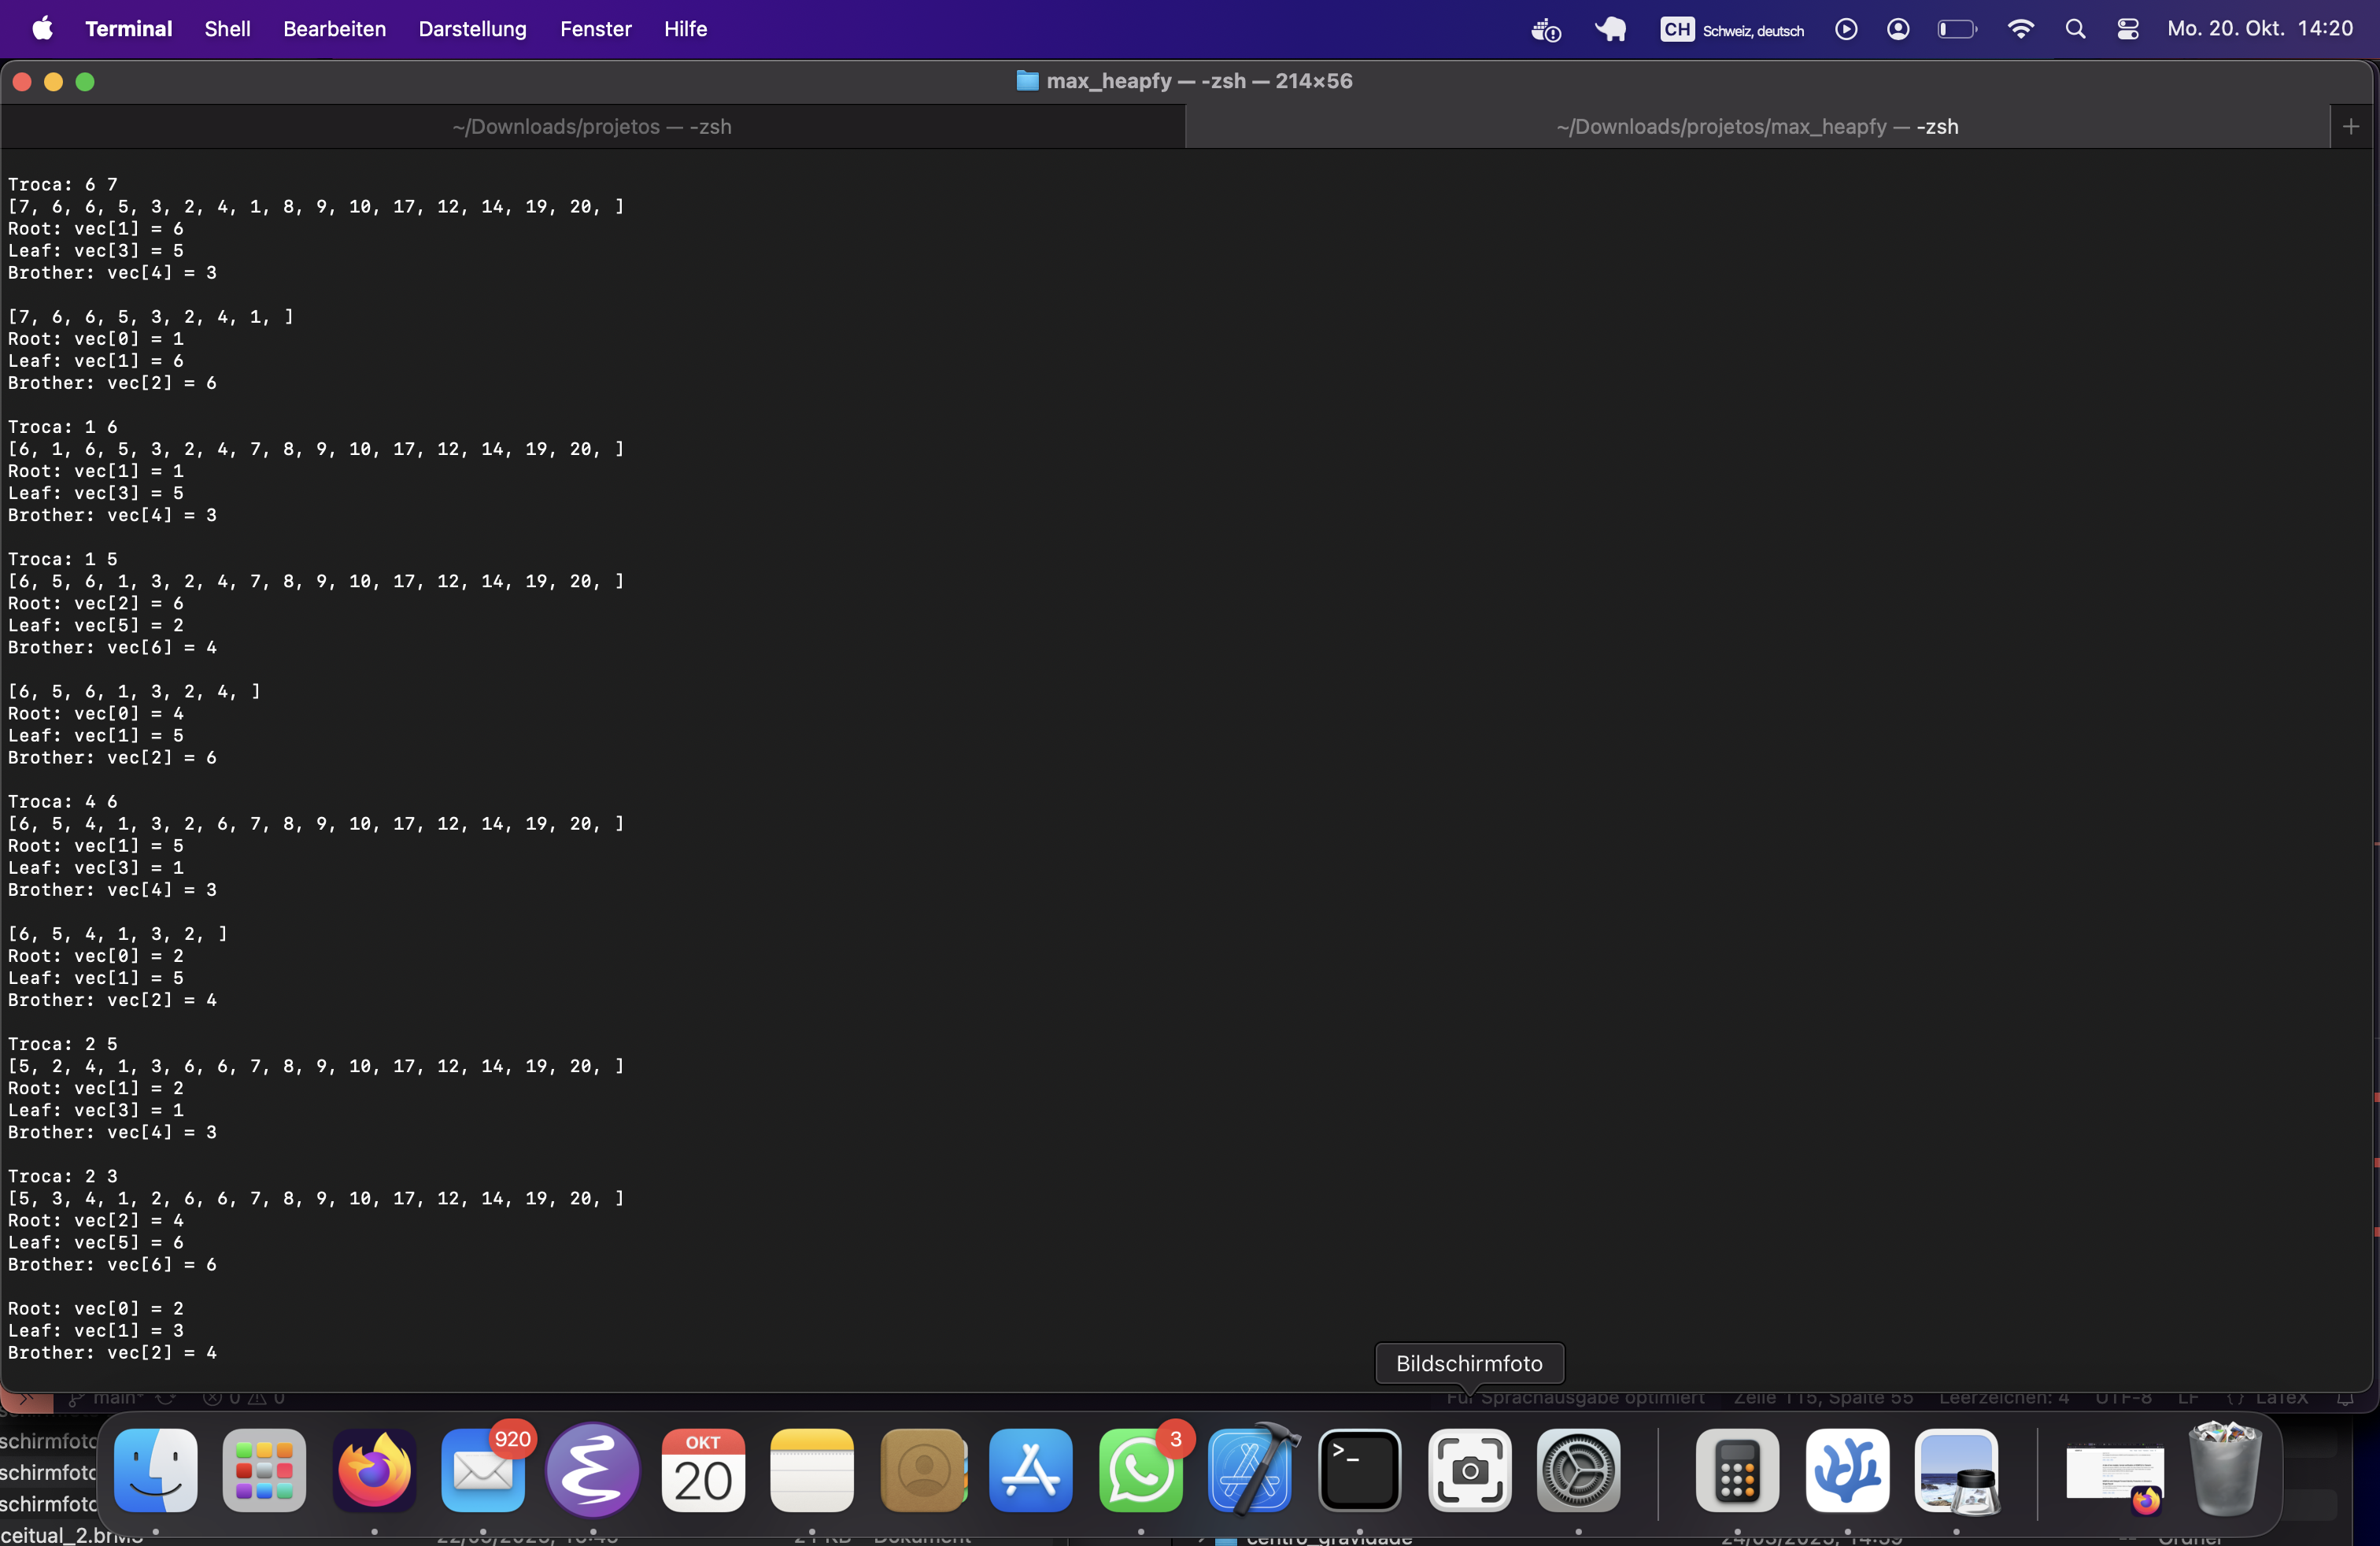
\includegraphics[width=1.3\linewidth]{heapsort3.png}
        \caption{Heap Sort, 3ª Página}
        \label{fig:myfig4}
    \end{figure}

    \begin{figure}
        \centering
        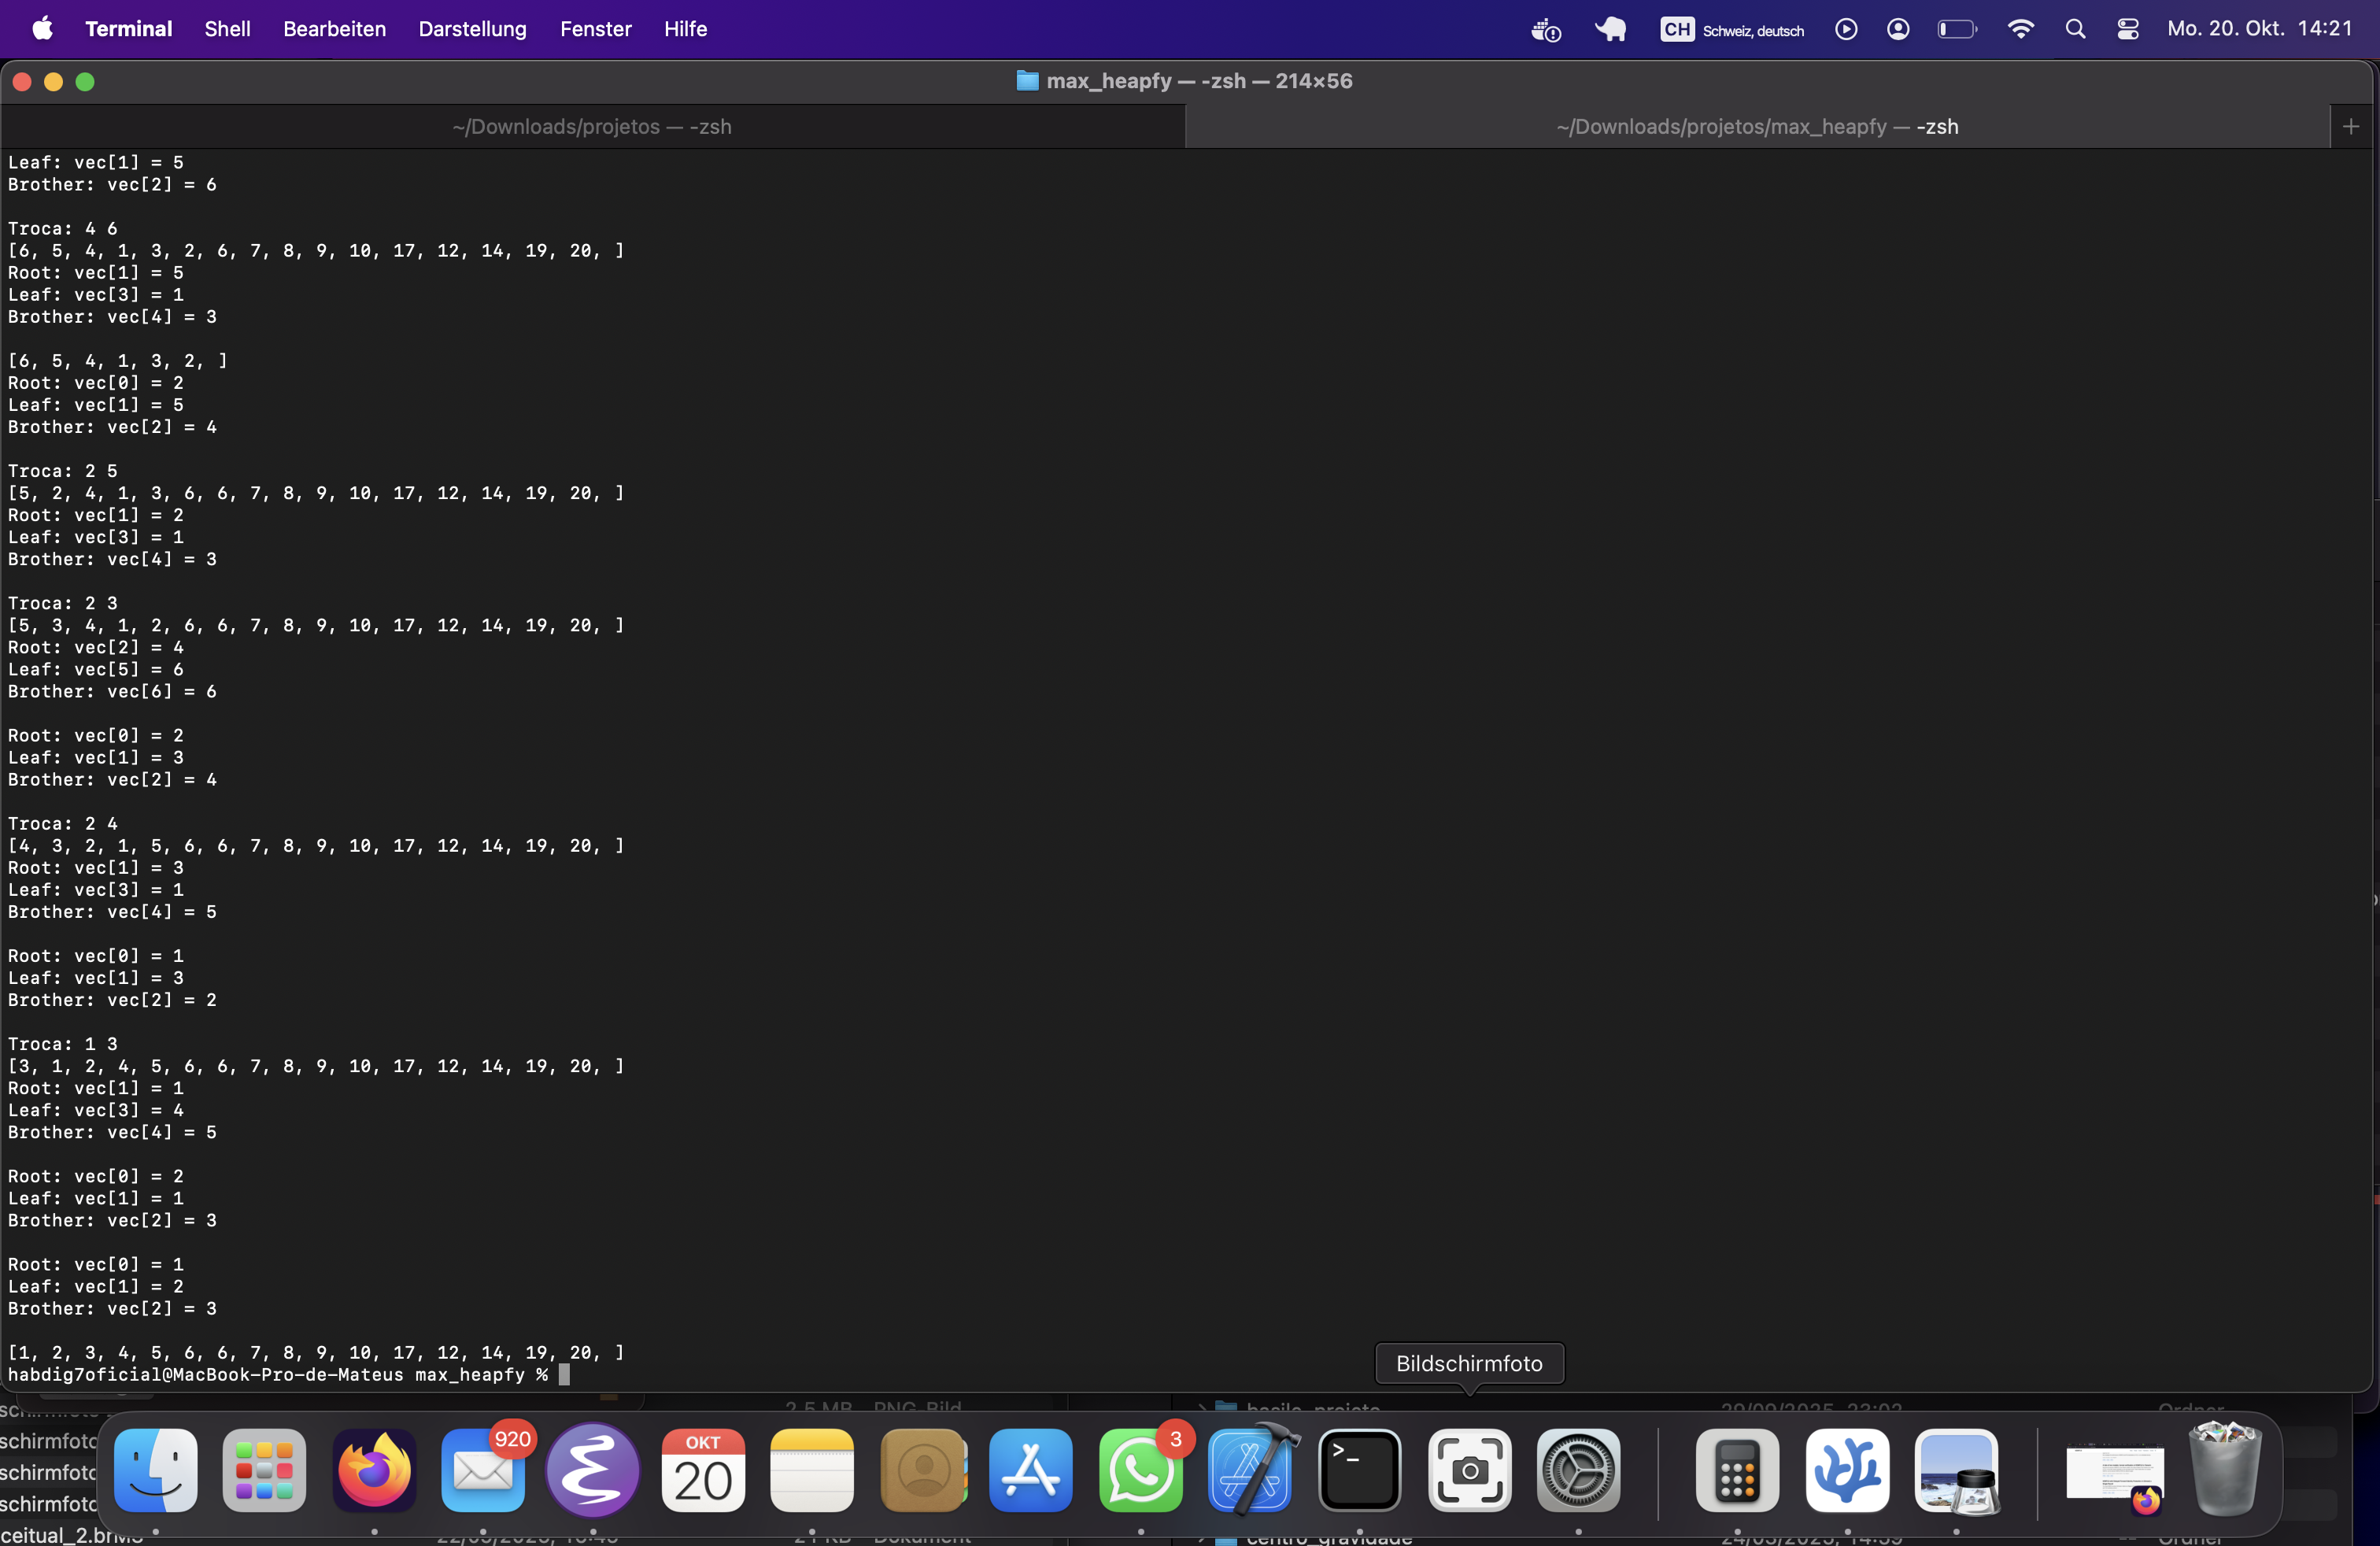
\includegraphics[width=1.3\linewidth]{heapsort4.png}
        \caption{Heap Sort, 4ª Página}
        \label{fig:myfig5}
    \end{figure}

    \clearpage

    \centerline{\Huge Code}

    \clearpage
    
    \begin{figure}
        \centering
        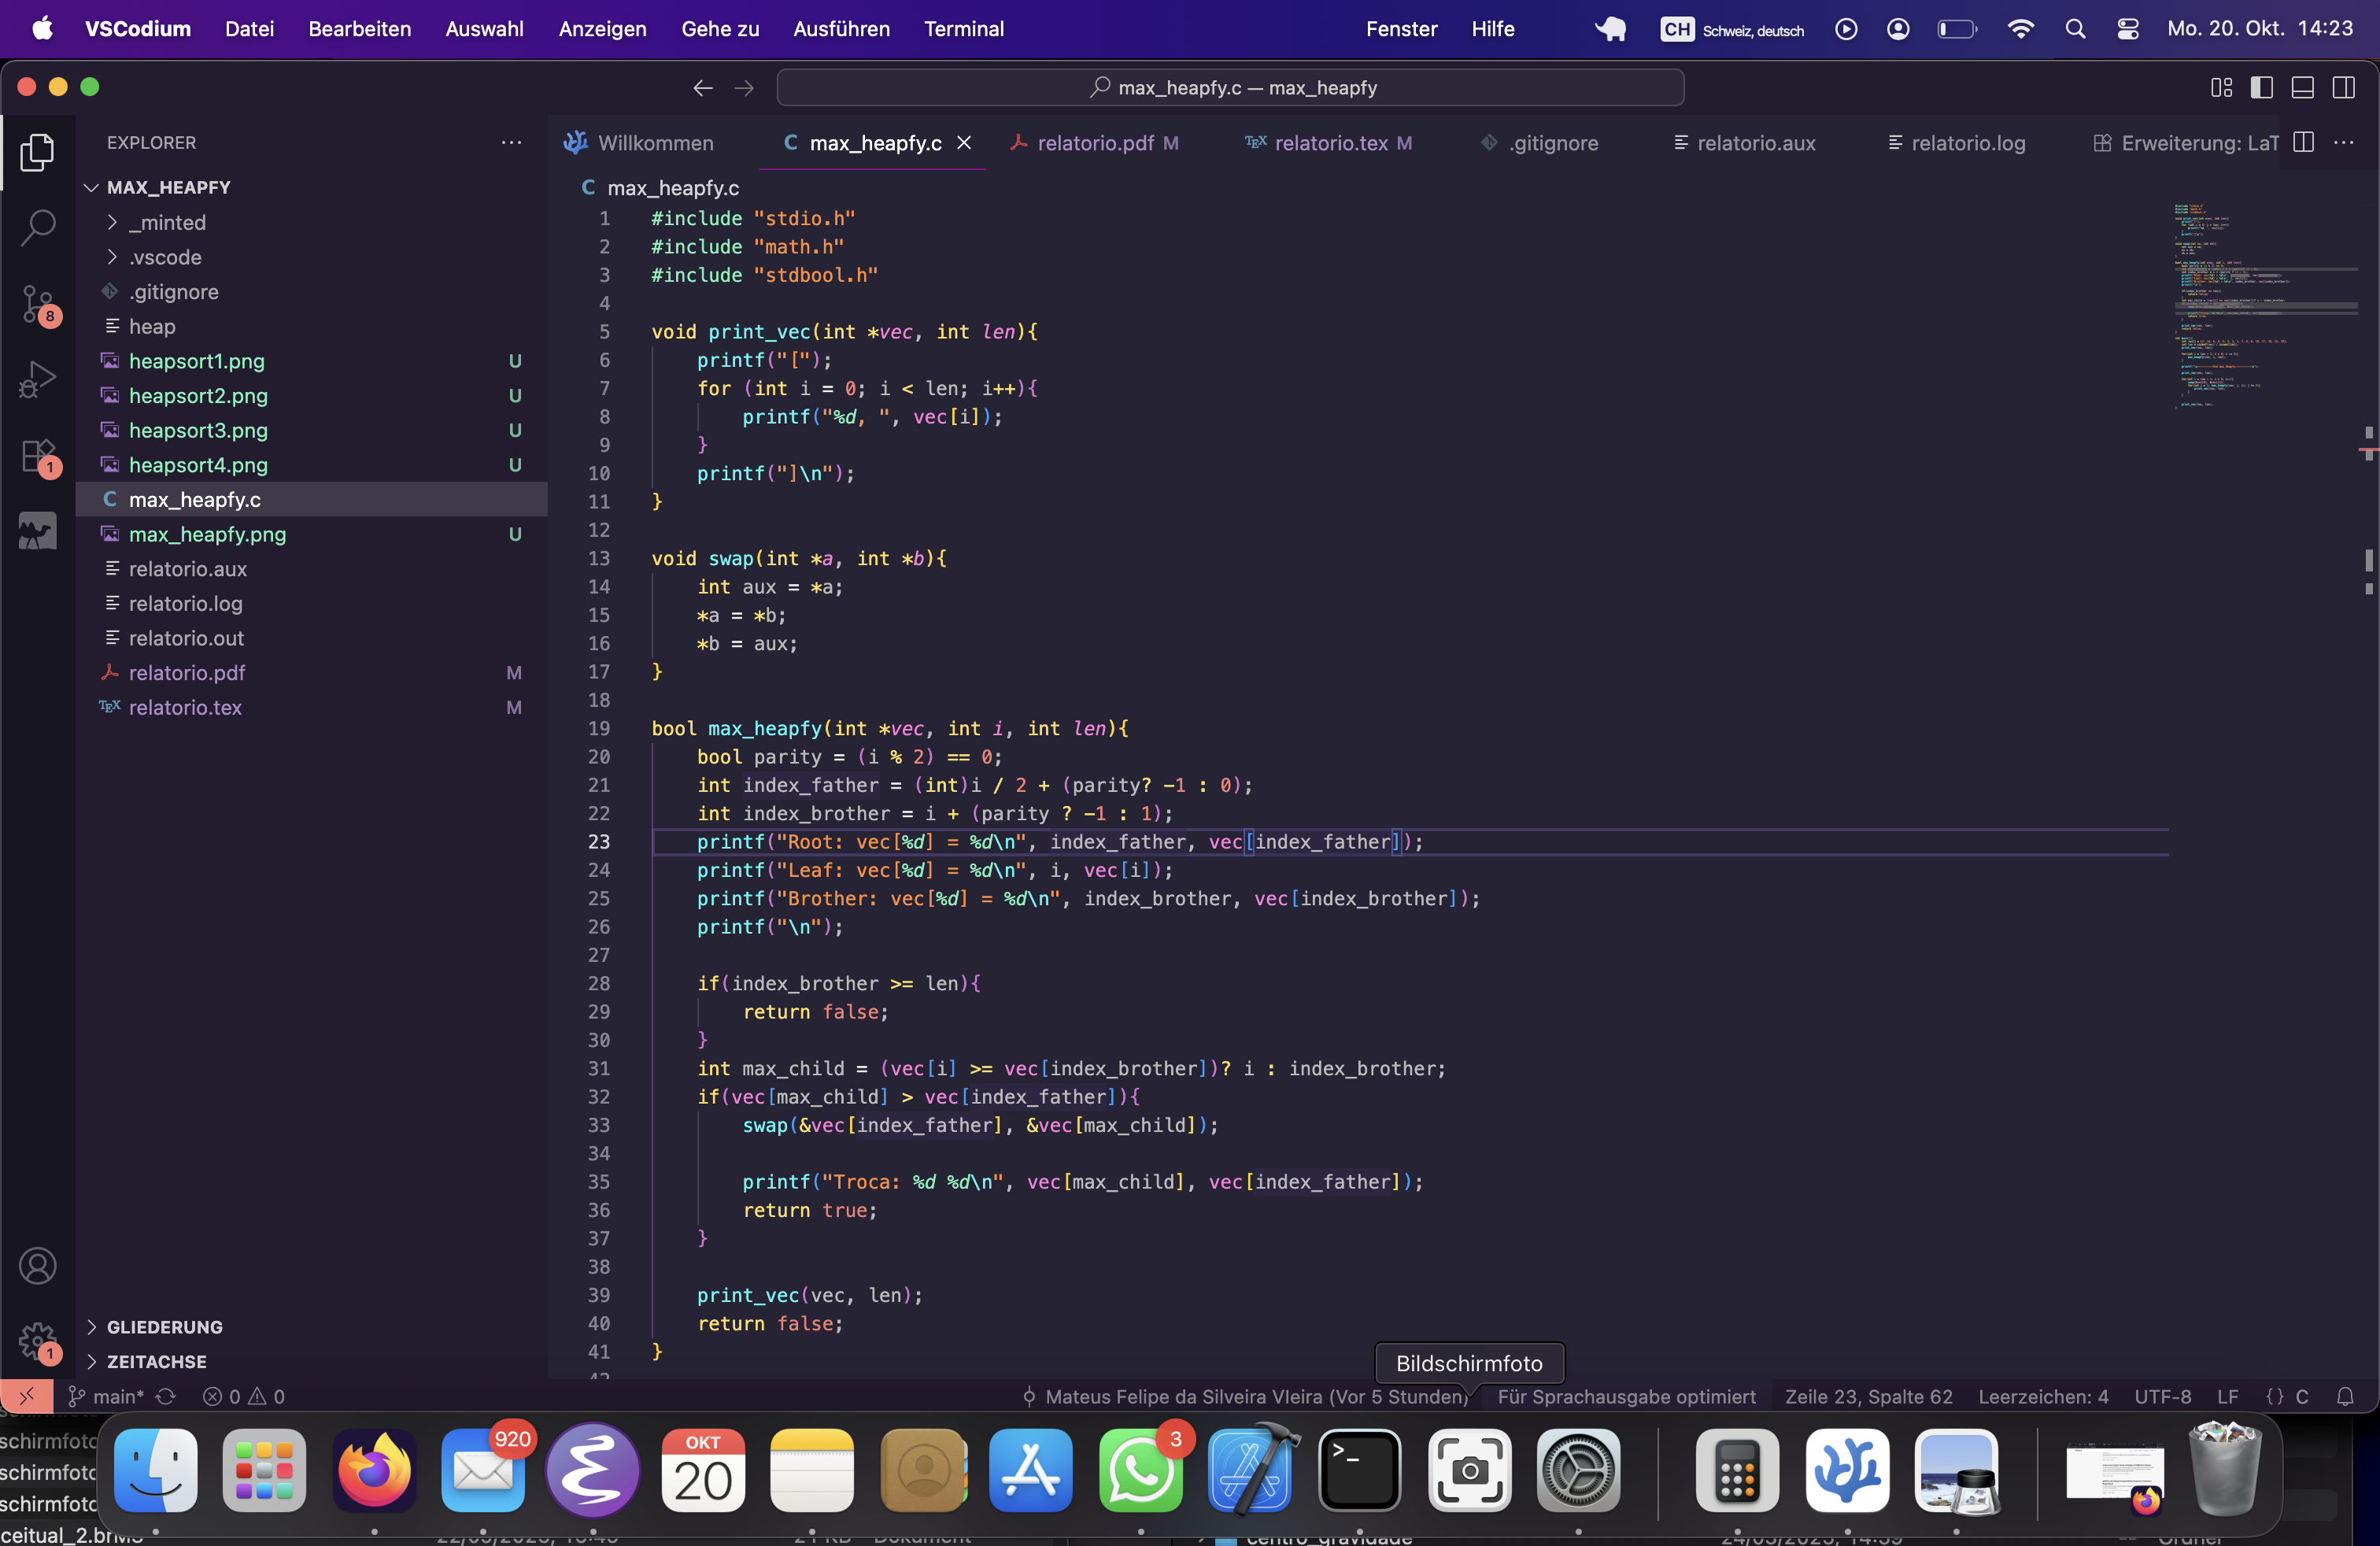
\includegraphics[width=1.3\linewidth]{code1.png}
        \caption{Code, 1ª Página}
        \label{fig:fig6}
    \end{figure}

    \begin{figure}
        \centering
        
\includegraphics[width=1.3\linewidth]{code2.png}
        \caption{Code, 2ª Página}
        \label{fig:fig6}
    \end{figure}

\end{document}